%%%%%%%%%%%%%%%%%%%%%%%%%
% Closure tests
%%%%%%%%%%%%%%%%%%%%%%%%%

% In this analysis, we do not explicitly estimate the background in the signal region from the
% observations in the control regions. Rather, 
% we create a prior distribution for the four background components of the signal regions, as
% described in Section~\ref{sec:likelihood},  that incorporates all
% statistical and systematic uncertainties. However,
% in order to verify that the control regions provide adequate data-driven models for
% the backgrounds in the signal region and that the translations between different regions behave as
% expected, we perform two cross checks, taking into account statistical uncertainties only. 
% 
% In the first cross check, we predict the background in a signal-like control region, denoted by
% $S^\prime$, defined by inverting the $\Delta\phi_{min}$ requirement while preserving the rest of the
% selection. 
% The estimated number of events in $S^\prime$ for the $t\bar{t}$ (plus single top), $\PW+$jets, and
% QCD multijet processes is computed as follows,
% \begin{equation}
%  \widehat{N}_{QCD}^{S^\prime} = \left( N_{obs}^{Q} - N_{other, MC}^{Q} \right)  / \left(
% \frac{N_{QCD}^{Q}}{N_{QCD}^{S^\prime}} \right)_{MC},
% \label{eq:E1}
% \end{equation}
% \begin{equation}
%  \widehat{N}_{\PW\ell\nu}^{S^\prime} = \left( N_{obs}^{W} - N_{other, MC}^{W} \right) / \left(
% \frac{N_{\PW\ell\nu}^{W}}{N_{\PW\ell\nu}^{S^\prime}} \right)_{MC},
% \label{eq:E2}
% \end{equation}
% \begin{equation}
%   \widehat{N}_{TTJ+T}^{S^\prime} = \left( N_{obs}^{T} - \widehat{N}_{QCD}^{T} - N_{other, MC}^{T}
% \right) / \left( \frac{N_{TTJ+T}^{T}} {N_{TTJ+T}^{S^\prime}}\right)_{MC},
% \label{eq:E3}
% \end{equation}
% while the estimated number of QCD events in the top control region is given by,
% \begin{equation}
%  \widehat{N}_{QCD}^{T} = \left( N_{obs}^{Q} - N_{other, MC}^{Q} \right) /  \left(
% \frac{N_{QCD}^{Q}}{N_{QCD}^{T}} \right)_{MC}.
% \label{eq:E4}
% \end{equation}
% As can be seen from Table~\ref{tab:cutflow}, $N_{QCD, MC}^{T} = 0$ for the nominal choice of
% systematic uncertainties. The formulae above can thus be simplified since $\widehat{N}_{QCD}^{T} =
% 0$. This is not necessarily the case for other choices of systematic variations, this relation is,
% therefore, still used to constrain the expected multijet background in the $T$ region during the
% final background estimate. 
% The total estimated background in $S^\prime$ is
% \begin{equation}
%   \hat{N}^{S^\prime} = \sum_i \hat{N}^{S^\prime}_i , 
% \end{equation}
% where $i$ runs over all background processes.  For the smaller backgrounds, $\hat{N}^{S^\prime}_i$
% is determined by simulation. 
% The estimation of backgrounds is done bin-by-bin in the $(\mathrm{M_R},\mathrm{R^2})$ space. 
% However, the estimated scale factors are global as the statistical precision is not sufficient to
% yield reliable bin-by-bin estimates. The expected global scale factors, which we denote by $\kappa$,
%  are defined in Section~\ref{sec:likelihood}, which also describes how they are calculated.
% 
% Figure~\ref{fig:Shape_syst_1D_project_sideband} shows the projection on the $\mathrm{M_R}$ and
% $\mathrm{R^2}$ axes of the predicted and observed distributions.  The prediction agrees with 
% observation within 20\%.  This cross check of the background modelling shows that it is feasible to
% estimate a multicomponent  background in a signal-like region using the control regions we
% have defined.
% 
% \begin{figure}[htpb]
% \includegraphics[width=0.5\textwidth]{figures/MR_comparison_data_estimate_g1Mbg1W0Ll_mdPhi0p5_log}
% \includegraphics[width=0.5\textwidth]{figures/R2_comparison_data_estimate_g1Mbg1W0Ll_mdPhi0p5_log}
% \caption{1D projection of $\mathrm{M_R}$ (left) and $\mathrm{R^2}$ (right) for the closure test
% predicting the $\Delta\phi_{min}$ sideband region $S'$. The uncertainties shown are statistical only
% and the horizontal error bars only indicate the bin width.
% \label{fig:Shape_syst_1D_project_sideband}}
% \end{figure}
% 
% In a second cross check, we use the $Q$ region to estimate the background in a signal-like $Q$
% region, denoted by $Q^\prime$, where $\Delta\phi_{min} > 0.5$, from the relationship
% \begin{equation}
%   \hat{N}^{Q^\prime} = N_{obs}^Q \frac{N_{MC}^{Q^\prime}}{N_{MC}^Q}.
% \end{equation}
% Here $N_{MC}$ includes all contributing background processes, and $N_{obs}^Q$ is the 
% observed count in the $Q$ region.
% The comparison between prediction and observations is shown in
% Fig.~\ref{fig:Shape_syst_1D_project_QCD}.
% Here, again, we  observe agreement within statistical uncertainties.  This test assesses 
% the degree to which the simulated distribution of $\Delta\phi_{min}$ as well as its extrapolation
% from the $Q$ region to the $S$ region are reliable. The level of discrepancy between the prediction
% and observations in this cross check is incorporated as a systematic uncertainty in the
% global scale factors, as described in Section~\ref{sec:likelihood}.
% 
% \begin{figure}[htpb]
% \includegraphics[width=0.5\textwidth]{
% figures/MR_comparison_data_estimate_0Lbg1uW0Ll_mdPhig0p5_from_0Lbg1uW0Ll_mdPhi0p3_log}
% \includegraphics[width=0.5\textwidth]{
% figures/R2_comparison_data_estimate_0Lbg1uW0Ll_mdPhig0p5_from_0Lbg1uW0Ll_mdPhi0p3_log}
% \caption{1D projection of $\mathrm{M_R}$ (left) and $\mathrm{R^2}$ (right) for the closure test
% predicting the background in region $Q'$ defined by $\Delta\phi_{min} > 0.5$.  The uncertainties
% shown are statistical only and the horizontal error bars only indicate the bin width.
% \label{fig:Shape_syst_1D_project_QCD}}
% \end{figure}




% 
% As illustrated in figure~\ref{fig:BoostWorkflow}, we use three control regions in our background
% prediction procedure. They are related to the signal region via translation factors determined in
% simulation. 
% The details of the control and signal region selection, and basic data/MC comparisons were shown in
% the previous sections. 
% In this section we will explain two cross-checks we performed in order to verify that the control
% regions are adequate and that the translation between different regions works. 
% To do this we will use two very simple methods, and take only statistical uncertainties into
% account. 
% 
% \subsubsection{Estimate the low $\Delta\phi_{min}$ sideband of the S region
% \label{sec:Shape_sideband}}
% 
% In order to check whether the basic background estimation method works, and to test several aspects
% of the MC modeling, we will predict the background in a region as close as possible to the signal
% region. 
% To achieve this, we take the signal region definition and invert the cut on  $\Delta\phi_{min}$. 
% This test will assess the following aspects of the MC modeling: btagging, $\Delta\phi_{min}$
% modeling for TTjets and Wjets, translation between lepton multiplicities, and certain aspects of the
% W-tagging. 
% 
% To speed up the process, we do not do the full likelihood based background estimation as we will do
% for the final results (and which is explained in section~\ref{sec:likelihood}), but approximate this
% by a simpler method. 
% The background in a given region $S'$ is composed of different processes. The total estimated
% background count in that region, $\hat{N}^{S'}$, can thus be written as: 
% \begin{equation}
%   \hat{N}^{S'} = \sum_i \hat{N}^{S'}_i , 
% \end{equation}
% where $i$ loops over all background processes. For the smaller backgrounds, $\hat{N}^{S'}_i$ is
% determined directly from the simulation. For the larger backgrounds we use control regions in data,
% denoted $Q$, $W$ and $T$. These control regions are the same as are used in the main background
% estimation. The estimated number of events in the signal sideband region for the TTjets (and single
% top), Wjets and QCD processes is computed as follows:
% \begin{equation}
%  \widehat{N}_{QCD}^{S'} = \left( N_{obs}^{Q} - N_{other, MC}^{Q} \right) \left(
% \frac{N_{QCD}^{S'}}{N_{QCD}^{Q}} \right)_{MC}
%  \label{eq:E1}
% \end{equation}
% \begin{equation}
%  \widehat{N}_{Wl\nu}^{S'} = \left( N_{obs}^{W} - N_{other, MC}^{W} \right) \left(
% \frac{N_{Wl\nu}^{S'}}{N_{Wl\nu}^{W}} \right)_{MC}\
%  \label{eq:E2}
% \end{equation}
% \begin{equation}
%   \widehat{N}_{TTJ+T}^{S'} = \left( N_{obs}^{T} - \widehat{N}_{QCD}^{T} - N_{other, MC}^{T} \right)
% \left( \frac{N_{TTJ+T}^{S'}}{N_{TTJ+T}^{T}} \right)_{MC}
%  \label{eq:E3}
% \end{equation}
% \begin{equation}
%  \widehat{N}_{QCD}^{T} = \left( N_{obs}^{Q} - N_{other, MC}^{Q} \right) \left(
% \frac{N_{QCD}^{T}}{N_{QCD}^{Q}} \right)_{MC}
%  \label{eq:E4}
% \end{equation}
% This estimation is done bin-by-bin in the $M_R$-$R^2$ plane. The MC ratios, however, are global
% ratios as the statistical precision is not sufficient to take them bin-by-bin as well. 
% In the current version of the analysis (since explicitely imposing $W p_T >200\GeV$), there is no
% QCD contribution in the $T$ region according to MC, $N_{QCD}^{T} = 0$, and these equations can thus
% be simplified. In the actual likelihood based background prediction, we can still have a non-zero
% $N_{QCD}^{T}$ due to effects of the systematic variations. 
% 
% The result of this estimation, a 2D prediction in the $M_R-R^2$ plane, can then be compared with the
% observation for that region in data. 
% As 2D histograms are hard to compare, we provide the 1D projections in
% figure~\ref{fig:Shape_syst_1D_project_sideband}. 
% From these we can see that there is a reasonable agreement, within about 20\%. 
% 
% \begin{figure}[htpb]
% \includegraphics[width=0.49\textwidth]{
% figures/ShapeSyst/MR_comparison_data_estimate_g1Mbg1W0Ll_mdPhi0p5_log}
% \includegraphics[width=0.49\textwidth]{
% figures/ShapeSyst/R2_comparison_data_estimate_g1Mbg1W0Ll_mdPhi0p5_log}
% \caption{1D projection of $M_R$ (left) and $R^2$ (right) for the closure test predicting the
% $\Delta\phi_{min}$ sideband of the S region. Uncertainties are statistical only.
% \label{fig:Shape_syst_1D_project_sideband}}
% \end{figure}
% 
% \subsubsection{Estimate the high $\Delta\phi_{min}$ sideband of the Q control region using the Q
% control region \label{sec:Shape_QCD}}
% 
% This test uses an even more basic method to validate the MC modeling.
% It uses this simple formula:
% \begin{equation}
%   \hat{N}^{A} = N_{obs}^B \frac{N_{MC}^A}{N_{MC}^B}
% \end{equation}
% with the Q control region (low $\Delta\phi_{min}$) taking the role of $B$, and the Q region with the
% cut on $\Delta\phi_{min}$ inverted (high $\Delta\phi_{min}$) taking the role of $A$. $N_{MC}$
% contains all background processes that contribute in that region. $N_{obs}$ is the data count in a
% given region. 
% 
% This closure tests checks the modeling of the $\Delta\phi_{min}$ variable for the QCD simulation. In
% the actual background prediction, we will use the extrapolation from the Q region, with low
% $\Delta\phi_{min}$, to the signal region, which has high $\Delta\phi_{min}$. This closure test thus
% assesses how well this extrapolation works. 
% 
% The comparison between prediction and observed data as 1D projections is shown in
% figure~\ref{fig:Shape_syst_1D_project_QCD}.
% Here we again observe reasonable agreement considering the statistical uncertainties. A flat 40\%
% systematic uncertainty will be applied to cover for the observed disagreement, see
% section~\ref{sec:shape_systematics}. 
% 
% \begin{figure}[htpb]
% \includegraphics[width=0.49\textwidth]{
% figures/ShapeSyst/MR_comparison_data_estimate_0Lbg1uW0Ll_mdPhig0p5_from_0Lbg1uW0Ll_mdPhi0p3_log}
% \includegraphics[width=0.49\textwidth]{
% figures/ShapeSyst/R2_comparison_data_estimate_0Lbg1uW0Ll_mdPhig0p5_from_0Lbg1uW0Ll_mdPhi0p3_log}
% \caption{1D projection of $M_R$ (left) and $R^2$ (right) for the closure test predicting the high
% $\Delta\phi_{min}$ region of the Q control region. \label{fig:Shape_syst_1D_project_QCD}}
% \end{figure}
% 
% 
% 
% 
